\section{Лекция номер 13}
\subsection*{После перерыва}
Сейчас нам понадобятся квадратичные формы.
Мы уже говорили о них на алгебре, но все равно вспомним основные определения и свойства.
\begin{conj}
    Функция называется квадратичная формой, если ее можно представить в виде $Q(h) = \sum\limits_{i, j = 1}^n c_{ij}h_ih_j$.
\end{conj}
Тут сумма $\sum\limits_{i, j = 1}^n c_{ij}h_ih_j$ это более корткая версия $\sum\limits_{i=1}^n\sum\limits_{j=1}^n c_{ij}h_ih_j$.

Обозначим матрицу коэффициентов за $C$.
Принято считать, что она симметричная: $c_{ij} = c_{ji}$.
Мы также можем написать следующее равенство: $Q(h) = \sum\limits_{i, j = 1}^n c_{ij}h_ih_j = \langle Ch, h \rangle$.
Это достаточно легко проверяется простым расписыванием, что на что умножается.

\begin{conj} Определенность квадратичной формы.

    \begin{itemize}
        \item $Q$ положительно определена, если $\forall h \in \R^n \;\; Q(h) \geqslant 0$.
        \item $Q$ отрицательно определена, если $\forall h \in \R^n \;\; Q(h) \leqslant 0$.
        \item $Q$ строго положительно определена, если $\forall h \neq 0 \in \R^n \;\; Q(h) > 0$.
        \item $Q$ строго отрицательно определена, если $\forall h \neq 0 \in \R^n \;\; Q(h) < 0$. 
    \end{itemize}
\end{conj}

\vspace*{5mm}

\begin{lemma}
    Если $Q(h)$ строго положительно определена, то $\exists c > 0$, т.ч. $Q(h) \geqslant c\|h\|^2 $
\end{lemma}
\begin{proof}
    Заметим, что $Q(h) = \langle Ch, h \rangle$ -- непрерывная функция.
    Давайте рассмотрим ее на единичной сфере (обобщение единичной окружности).
    Это компактное множество, а мы знаем, что непрерывная функция на компакте обязана принимать свое минимальное значение: $\exists h_0 : \|h_0\| = 1$ и $Q(h) \geqslant Q(h_0) \;\; \forall h : \|h\| = 1$.
    
    Положим $c = Q(h_0)$ и докажем, что оно подходит.
    Все, что нам надо сделать, это просто отнормировать вектор и воспользоваться неравенством: \[ \forall h \;\; Q(h) = \langle Ch, h \rangle = \|h\|^2 \left\langle C \frac{h}{\|h\|}, \frac{h}{\|h\|} \right\rangle = \|h\|^2Q\left(\frac{h}{\|h\|}\right) \geqslant c\|h\| \]
\end{proof}

\begin{theorem} [достаточные условия экстремума]
    Пусть $f: E \to \R$, $a$ -- стационарная точка, $f$ дважды дифференцируема в точке $a$, $Q(h) = \sum\limits_{i, j = 1}^n f''_{x_ix_j}(a)h_ih_j$ -- квадратичная форма. Тогда: \begin{enumerate}
        \item Если $Q$ строго положительно (отрицательно) определена, то $a$ -- строгий локальный минимум (максимум).
        \item Если $a$ -- нестрогий локальный минимум (максимум), то $Q$ нестрого положительно (отрицательно) определена.
    \end{enumerate}
\end{theorem}
\begin{proof} \quad
    \begin{enumerate}
        \item Будем доказывать для минимума.
        Воспользуемся формулой Тейлора для стационарной точки: \begin{gather*}
            f(a + h) = f(a) + \frac{1}{2} \sum_{i, j = 1}^n f''_{x_ix_j}(a)h_ih_j + o(\|h\|^2) \\
            \Rightarrow f(a + h) - f(a) = \frac{1}{2}Q(h) + o(\|h\|^2) = \frac{1}{2}Q(h) + \alpha(h)\|h\|^2, \text{ где } \alpha(h) \to 0 \text{ при } h \to 0
        \end{gather*}
        Воспользуемся леммой: \[ f(a+h) - f(a) =  \frac{1}{2}Q(h) + \alpha(h)\|h\|^2 \geqslant \frac{c}{2}\|h\|^2 + \alpha(h)\|h\|^2 = \|h\|^2 \left(\frac{c}{2} - \alpha(h) \right)  \]
        Осталось заметить, что при малых $h$ множитель $(\frac{c}{2} - \alpha(h)) > 0$, следовательно, $f(a + h) - f(a) > 0$, а это означает, что $a$ -- строгий локальный минимум.
        \item Опять же будем доказывать только для минимума. 
        Зафиксируем произвольное $h$.
        Мы хотим показать, что $Q(h) \geqslant 0$. 
        Воспользуемся все той же формулой Тейлора, но только теперь, так как $h$ фиксировано, введем вспомогательный параметр $t$:
        \[ f(a + th) - f(a) = \frac{1}{2}Q(th) + \underbrace{o(t^2\|h\|^2)}_{= o(t^2)} \]
        Вынесем $t$ из под квадратичной формы (в каждом слагаемом у нас есть умножение на $t^2$): 
        \begin{gather*}
            f(a + th) - f(a) = t^2 \left(\frac{Q(h)}{2} + o(1) \right) \\
            \frac{f(a + th) - f(a)}{t^2} = \frac{Q(h)}{2} + o(1)
        \end{gather*}
        Вследствие того, что $a$ -- локальный минимум, выражение $\frac{f(a + th) - f(a)}{t^2} \geqslant 0$.
        Устремим $t$ к нулю, чтобы убрать $o(1)$, и получим, что $\frac{Q(h)}{2} \geqslant 0$.
    \end{enumerate}
\end{proof}

\notice \, Если $Q$ не имеет нестрогую знакоопределенность, то $a$ не точка экстремума.

\vspace*{5mm}

А как по матрице квадратичной формы понять, что она положительно определена? Или строго положительно?
На этот вопрос помогает ответить критерий Сильвестра, который мы оставим без доказательства.

\textbf{Критерий Сильвестра.} Путь $Q(h) = \langle Ch, h \rangle$. 
Тогда чтобы понять определенность $Q$, надо посмотреть на последовательность знаков определителей следующих миноров: \begin{gather*}
    \begin{vmatrix}
        c_{11}
    \end{vmatrix}, \begin{vmatrix}
        c_{11} & c_{12} \\
        c_{21} & c_{22}
    \end{vmatrix}, \begin{vmatrix}
        c_{11} & c_{12} & c_{13} \\
        c_{21} & c_{22} & c_{23} \\
        c_{31} & c_{32} & c_{33}    
    \end{vmatrix}, \dots, \begin{vmatrix}
        c_{11} & \dots & c_{1n} \\
        \dots & \dots & \dots \\
        c_{n1} & \dots & c_{nn} 
    \end{vmatrix}
\end{gather*} 
\begin{itemize}
    \item Если они все $> 0$, то форма строго положительно определена.
    \item Если они все $\geqslant 0$, то форма положительно определена.
    \item Если они образуют знакочередующуюся последовательность, начинающуюся с отрицательного числа, то мы можем говорить про (строгую, если все знаки строгие) отрицательную определенность.
\end{itemize}

\begin{example}
    Найдем экстремумы у функции $f(x, y) = x^4 + y^4 - 36xy$.

    Для начала надо найти стационарные точки.
    Функция везде дифференцируемая, так что надо просто найти точки, в которых градиент равен 0: \begin{gather*}
        \begin{cases}
            f'_x(x, y) = 4x^3 - 36y = 0 \\
            f'_y(x, y) = 4y^3 - 36x = 0
        \end{cases}
    \end{gather*}
    Несложно проверить, что это будут точки $\{ (3, 3), (-3, -3), (0, 0) \}$.
    Чтобы посчитать нужную квадратичную форму, нам нужны вторые производные: \begin{gather*} 
        f''_{xx}(x, y) = 12x^2 \quad f''_{yy}(x, y) = 12y^2 \quad f''_{xy}(x, y) = f''_{yx}(x, y) = -36 \\
        \Rightarrow Q(x, y) = \begin{pmatrix}
            12x^2 & -36 \\
            -36 & 12y^2
        \end{pmatrix}
    \end{gather*}
    Осталось подставить конкретные точки и по критерию Сильвестра определить, какая у нас форма: \begin{itemize}
        \item Для точки $(3, 3)$ последовательность определителей выглядит как $\{ 9, 72 \}$, значит форма строго положительно определена, и $(3, 3)$ -- строгий минимум.
        \item Для точки $(-3, -3)$ все аналогично.
        \item Для точки $(0, 0)$ получаем последовательность $\{ 0, -9 \}$, значит, форма не имеет нестрогую знакоопределенность, и $(0, 0)$ не точка экстремума.
    \end{itemize}
\end{example} 

\vspace*{5mm}

Почему не все точки, у которых частные производные 0, являются экстремумами?
Может так оказаться, что по одним координатам точка является локальным минимумом, а по другим -- локальным максимумом.
Такие точки называются седловыми. 
Ниже представлен пример для $f(x, y) = x^2 - y^2$.

\begin{center}
    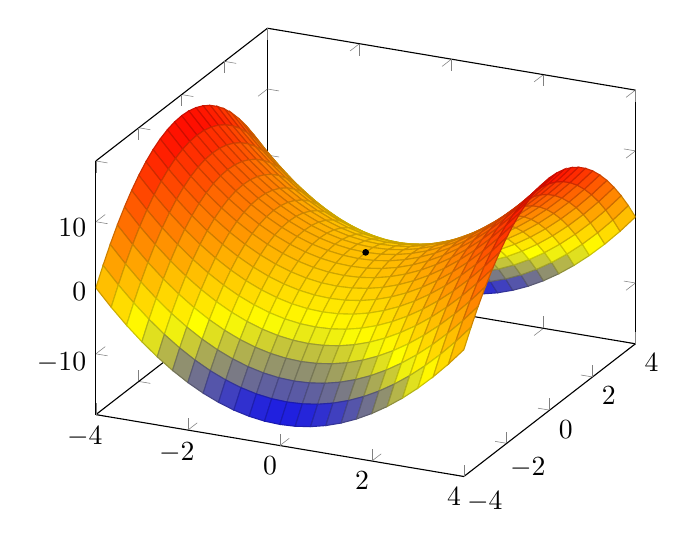
\begin{tikzpicture}
        \begin{axis}
            \addplot3 [
                surf,
                shader=faceted,
                samples=25,
                domain=-4:4,
                y domain=-4:4
                ] {x^2-y^2};
            \filldraw[black] (axis cs:0,0,0) circle(1pt);
        \end{axis}
    \end{tikzpicture}
\end{center}

Зачастую нас интересуют не локальные, а глобальные экстремумы.
Возникает логичный вопрос, как их искать?
Казалось бы, что достаточно найти все стационарные точки и сравнить значние в них.
Тогда самое большое/маленькое и будет глобальным максимумом/минимумом.
Но заметим, что если мы рассматриваем функцию на компакте, то мы обязаны рассмотреть ее и на границе, но стационарные точки определяются как внутренние.
То есть вдруг окажется так, что максимум/минимум лежит на границе?
Поэтому надо научиться справляться с точками на границе.

Иногда бывает также полезно искать экстремумы у функции, заданной на какой-то поверхности.
Например, функция температуры на планете задана на сфере, а вовсе не в $\R^3$.

Чтобы понять, как нам все это искать, введем определение условного экстремума.

\begin{conj}
    Пусть у нас есть:
    \begin{gather*}
        f: D \subset \R^{n+m} \to \R, \Phi: D \to \R^m, a \in D \text{ и } \Phi(a) = 0
    \end{gather*}
    Если существует $U$ окр-ть точки $a$, т.ч $\forall x \in U \cap D$ и $\Phi(x) = 0$, будет $f(x) \leqslant f(a)$, то $a$ -- нестрогий условный максимум при условии связи $\Phi = 0$.
    Точно также можно определить строгий максимум и аналогично минимум.
\end{conj}

Разберем это на примере.
У нас есть функция $f(x, y) = x^2 + y^2$ (оранжевый график).
Зададим функцию $\Phi(x, y) = x - 20$.
Точки, удовлетворяющие уравнению $\Phi = 0$ и лежащие на графике функции, будут образовывать зеленую кривую. 
Тогда точка $(20, 0, 400)$ будет строгим условным минимумом при условии связи $\Phi = 0$.

\begin{center}
    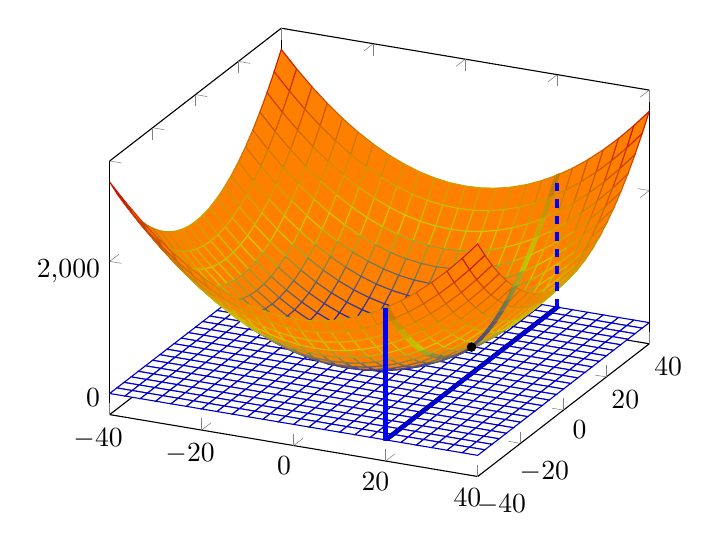
\begin{tikzpicture}
        \begin{axis} 
            \addplot3 [
                surf,
                white,
                shader=faceted,
                domain =-40:40,
                y domain=-40:40
                ] {0};

            \addplot3 [
                surf,
                orange,
                shader=faceted,
                samples=25,
                domain =-40:40,
                y domain=-40:40
                ] {x^2+y^2};

                \addplot3 [
                surf,
                black,
                shader=faceted,
                domain =19.5:20.5,
                y domain=-40:40
                ] {x^2+y^2};

                \addplot3 [
                surf,
                black,
                shader=faceted,
                domain =19.5:20.5,
                y domain=-40:40
                ] {0};

                \draw[blue, ultra thick] (axis cs:20, -40, 0) -- (axis cs:20, -40, 2000);

                \draw[blue, ultra thick, dashed] (axis cs:20, 40, 0) -- (axis cs:20, 40, 2000);
                
                \filldraw[black] (axis cs:20,0,400) circle(1.5pt);
    
        \end{axis}
    \end{tikzpicture}
\end{center}


Теперь нас интересует способ найти какие-то необходимые условия на условные экстремумы.
Для этого существует метод неопределенных множителей Лагранжа.

\vspace*{5mm}

\textbf{Метод множителей Лагранжа.} 

\textit{(тут возможно есть некоторое кол-во ошибок, в скором времени они будут исправлены)}

Пусть $f: D \subset \R^{n+m} \to \R$ непрерывно дифференцируема, $ \Phi: D \to \R^m$ непрерывно дифференцируема, $a \in \Int D$.
Тогда если $a$ точка условного экстремума при условии связи $\Phi = 0$, то $\nabla f, \nabla \Phi_1, \nabla \Phi_2, \dots, \nabla \Phi_m$ в точке $a$ линейно зависимы.

\notice \begin{enumerate}
    \item Если $\nabla \Phi_1, \nabla \Phi_2, \dots, \nabla \Phi_m$ линейно независимы, то существуют $\lambda_1, \dots, \lambda_m \in \R$, т.ч. $\nabla f = \lambda_1 \nabla \Phi_1 + \dots + \lambda_m \nabla \Phi_m$.
    Это просто по определению: у нас была ЛНС, добавили 1 вектор, стала ЛЗС $\Rightarrow$ можем выразить в виде линейной комбинации.
    \item Что означает линейная независимость $\nabla \Phi_1, \nabla \Phi_2, \dots, \nabla \Phi_m$?
    Вспоним, что эти градиенты -- строки матрицы Якоби $\Phi$ в точке $a$ (у этой матрицы $m$ строк и $n+m$ столбцов).
    Таким обоазом, это означает, что $rk\, \Phi'(a) = m$.
    
    Мы также можем упростить запись в первом пукнте, если представим лямбды как вектор-строку: $\lambda = (\lambda_1, \dots, \lambda_m) \Longrightarrow \nabla f = \lambda_1 \nabla \Phi_1 + \dots + \lambda_m \nabla \Phi_m = \lambda \Phi'(a)$.
\end{enumerate}

\begin{proof}
    Ранг $\Phi'(a) = n$ и надо доказать, что $f'(a) = \lambda \Phi'(a)$ для некоторого $\lambda \in \R^m$.

    Считаем, что минор $\Phi'(a)$ по последним координатам $\neq 0$.
    Мы всегда можем этого добиться, просто попереставляв их. 
    Будем обозначать $a = (b, c)$, где $c$ как раз и будут последними координатами.
    Так как там минор $\neq 0$, есть обратимость, а значит, мы можем применить теорему о неявно заданной функции.
    Согласно ней $\exists W$ окр-ть точки $b$ и непрерывно дифференцируемая функция $g: W \to \R^m$, т.ч. $g(b) = c$ и $\Phi(x, g(x)) = 0 \;\; \forall x \in W$.

    Введем \begin{gather*}
        h(x): W \to \R^m \\ h(x) = f(x, g(x))
    \end{gather*} 
    Заметим, что $b$ будет экстремумом для $h$, так как при $x$ близком к $b$ у нас $g(x)$ будет близко к $c$, таким образом $(x, g(x))$ будет близко к $a$. А это условный экстремум по условию.

    В силу необходимого условия экстремума получаем, что $h'(b) = 0$.
    Давайте посчитаем эту производную. 
    Для этого разобьем матрицу из частичных производных $f(a)$ на 2: $f'_x(a)$ -- матрица из частных производных по первым координатам, $f'_y(a)$ -- матрица из частных производных по последним координатам.
    Тогда: \[ h'(b) = f'_x(a) + f'_y(a) \cdot g'(b) = 0 \]
    Мы также знаем, что $\Phi(b, g(b)) \equiv 0$, производная 0 равно 0, поэтому: \[ \Phi'(b, g(b)) = \Phi_x'(a) + \Phi_y'(a)\cdot g'(b) = 0  \]
    Вычтем из $h'(b)$ последнее выражение, домноженное на произвольное $\lambda \in \R^m$ : \[ (f'_x(a) - \lambda \Phi_x'(a)) + (f'_y(a) - \lambda \Phi_y'(a))\cdot g'(b) = 0  \]
    Осталось правильным образом выбрать $\lambda$. 
    Давайте выберем ее так, что $f'_y(a) - \lambda \Phi_y'(a) = 0$. 
    Мы так можем сделать, потому что  минор $\Phi'(a)$ по последним координатам $\neq 0$, а $y$ это как раз и есть последние координаты.
    Поэтому уравнение $f'_y(a) - \lambda \Phi_y'(a) = 0$ будет разрешимо относительно $\lambda$.

    Мы занулили второе слагаемое, поэтому обязано занулиться и первое: $f'_x(a) - \lambda \Phi_x'(a) = 0$.
    Если объединить эти результаты, то получится, что: \[ f'(a) = \lambda \Phi'(a) \]
    Что и требовалось доказать.
\end{proof}

\vspace*{5mm}

Осталось понять, как искать такие $a$.
В уравнении $f'(a) = \lambda \Phi'(a)$ у нас $2m + n$ неизвестных: $n + m$ координат точки $a$ и $m$ координат $\lambda$.
Посмотрим на число уравнений. 
Уравнение $f'(a) = \lambda \Phi'(a)$ распадается на $n + m$ штук (по каждой координате $a$).
Также точка $a$ обязана удовлетворять уравнению $\Phi(a) = 0$, что дает еще $m$ уравнений.
Таким образом, чтобы найти $a$ и $\lambda$ надо решить систему из $2m + n$ уравнений от такого же количества неизвестных. 
 
\vspace*{5mm}

\begin{conj}
    Функция Лагранжа -- функция, которая в наших предыдущих обозначениях равна $f - \lambda \Phi$.
    Таким образом, чтобы найти условные экстремумы, надо искать точки, где производная функции Лагранжа нулится.
\end{conj}

\vspace*{5mm}

Обсудим поясняющий пример.

\textbf{Наибольшее и наименьшее значения квадратичной формы на сфере.}

    Квадратичная форма задается симметричной матрицей $A$: $Q(h) = \langle Ah, h \rangle$.

    Сфера задается уравнением $x_1^2 + \dots + x_n^2 = 1$.
    Значит, $\Phi(x) = x_1^2 + \dots + x_n^2 - 1$.

    Пишем функцию Лагранжа: \[ F(x) = \sum_{i, j = 1}^n a_{ij}x_ix_j - \lambda(x_1^2 + \dots + x_n^2 - 1) \]
    Нас интересует такая точка, в которой $\Phi = 0$, и все частные производные $F$ равны 0.

    Распишем, чему равна $k$-тая частная производная $F$ (мы фиксируем $x_k$, остальное воспринимаем как параметры): \[ F_{x_k}' = a_{kk}*2x_k + \sum_{i\neq k} a_{ik}x_i + \sum_{j \neq k} a_{kj}x_j -2\lambda x_k = \circledast \]
    Заметим, что так как матрица $A$ симметричная, выражение можно упростить: \[ \circledast = 2\sum_{i = 1}^n a_{ki}x_i - 2\lambda x_k \]
    Что такое $\sum\limits_{i = 1}^n a_{ki}x_i$? 
    Это ни что иное как $k$-ая координата вектора $Ax$. 
    Таким образом, все координаты вектора $2Ax$ равны координатами вектора $2\lambda x$, или чуть короче: \[ Ax = \lambda x \]
    Это означает, что $x$ -- собственный вектор матрицы $A$ с собственным значением $\lambda$.
    Таким образом, точки, которые подозрительные на экстремум, обязаны быть собственными векторами матрицы.
    
    Также легко понять, какие значения принимает форма на этих векторах: \[ Q(x) = \langle Ax, x \rangle = \langle \lambda x, x \rangle = \lambda \| x \|^2 = \lambda  \]
    Последний переход верен, так как $x$ лежит на единичной сфере.
    Из этих рассуждений следует логичный вывод.

\begin{theorem}
    Наибольшее (наименьшее) значение квадратичной формы на сфере -- наибольшее (наименьшее) собственное число ее матрицы.
\end{theorem}

\vspace*{5mm}

\follow $\, \| A \| = \max \{ \sqrt{\lambda} : \lambda - \text{ собственное число матрицы } A^TA \}$.
\begin{proof}
    По определению нормы $\|A\| = \max\limits_{\|x\| = 1} \|Ax\|^2 = \max\limits_{\|x\| = 1} \langle Ax, Ax \rangle$.
    
    Воспользуемся алгебраическим фактом: $\langle Ax, Ax \rangle = \langle A^TAx, x \rangle$.
    А ведь $\max\limits_{\|x\| = 1} \langle A^TAx, x \rangle$ это и есть наибольшее значение квадратичной формы для матрицы $A^TA$ на единичной сфере.
\end{proof}



